\documentclass[tikz, varwidth=600pt]{standalone}
\usepackage{amssymb, amsmath,bbm}

\standaloneenv{aaaa}

\begin{document}
	\begin{aaaa}
		\begin{center}	
		
		\fbox{%
			\begin{minipage}{0.85\linewidth}
				\centering
				\tikzset{every picture/.style={line width=0.75pt}} %set default line width to 0.75pt        
				\vspace{6pt} 
		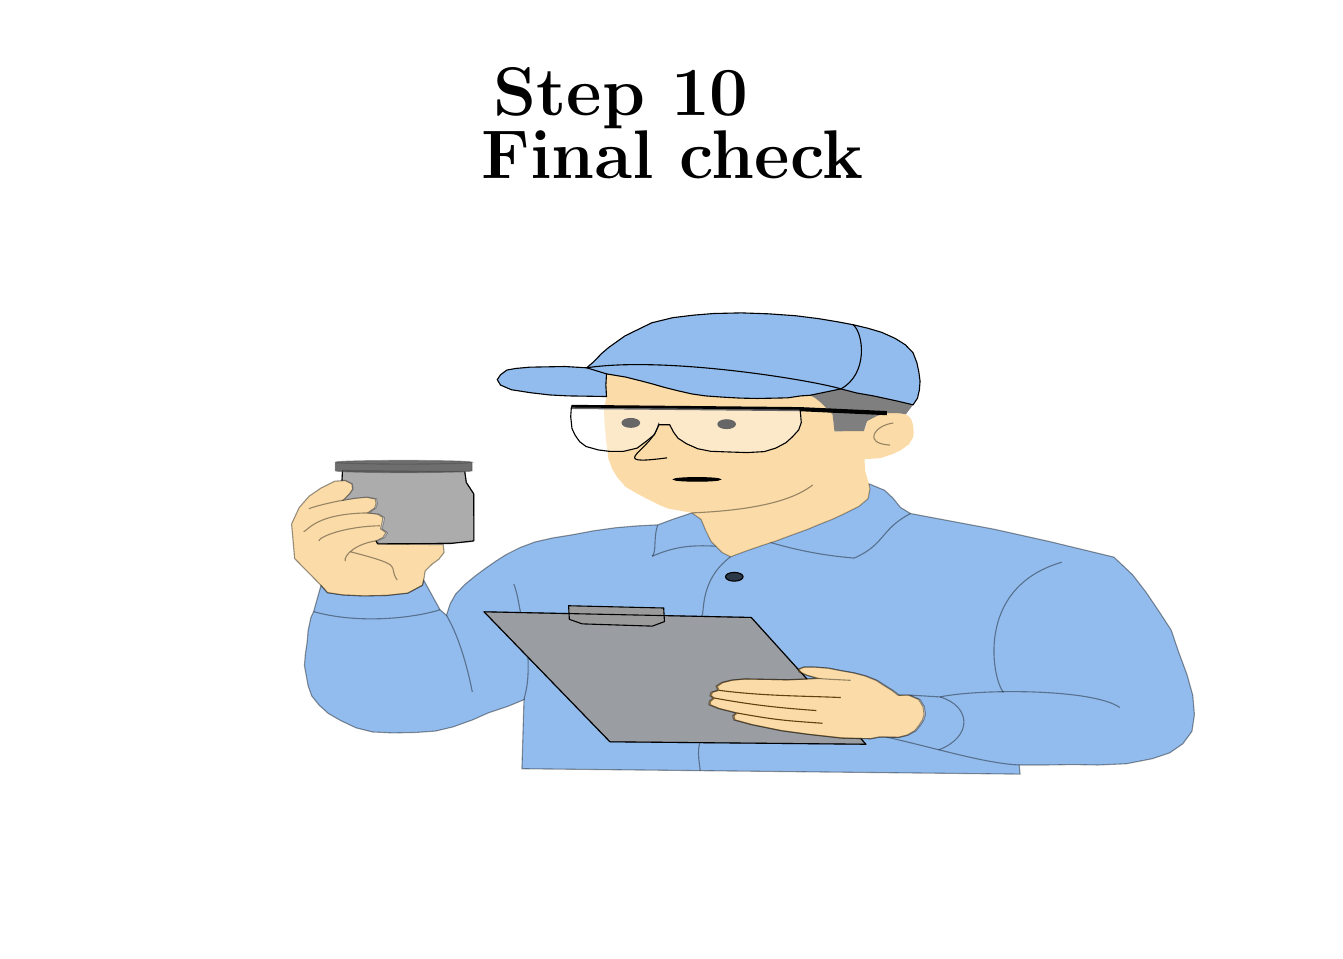
\begin{tikzpicture}[x=0.75pt,y=0.75pt,yscale=-1,xscale=2]
			%uncomment if require: \path (0,419); %set diagram left start at 0, and has height of 419
			
			\path[use as bounding box] (20,5) rectangle (330,440);
			
			
			\begin{scope}[xshift=-100, yshift=-95]
			%Shape: Path Data [id:dp5422614003673734] 
			\draw  [color={rgb, 255:red, 0; green, 0; blue, 0 }  ,draw opacity=0.4 ][fill={rgb, 255:red, 74; green, 144; blue, 226 }  ,fill opacity=0.6 ] (366,365.75) -- (386,373.25) -- (399.5,379.25) -- (415,386.75) -- (419.5,395.25) -- (422.67,403.44) -- (425.6,412.1) -- (428.8,421.9) -- (430.6,432.5) -- (432.6,443.3) -- (434,453.3) -- (434.4,462.7) -- (433.8,470.7) -- (431.6,476.7) -- (428.4,481.1) -- (424.2,483.9) -- (418,486.3) -- (411.2,486.9) -- (405.2,486.7) -- (398.8,486.9) -- (392.2,486.9) -- (392.4,491.3) -- (272.4,488.7) -- (272.89,455.44) -- (269.11,458.56) -- (264.44,461.67) -- (260.44,465.22) -- (255.78,468.56) -- (251.56,470.56) -- (246.89,471.22) -- (241.33,471.44) -- (236.44,471) -- (232.44,469) -- (228.89,465.67) -- (225.78,462.11) -- (223.56,458.11) -- (221.78,453.67) -- (220.89,448.78) -- (220,439) -- (220.22,433.67) -- (220.67,427.44) -- (220.89,422.11) -- (221.56,415.89) -- (222.22,413) -- (224,400.36) -- (225.56,403.89) -- (229.33,405) -- (234.22,405.44) -- (239.78,405.22) -- (244.89,404.11) -- (248.44,400.33) -- (248.73,397.82) -- (252.67,412.11) -- (254.22,414.78) -- (255.11,409.22) -- (256.44,404.56) -- (258.67,399.89) -- (261.11,395.89) -- (263.33,392.56) -- (266.22,388.56) -- (268.67,385.44) -- (272,382.11) -- (275.56,379.44) -- (280,377.44) -- (284.22,376.11) -- (289.56,374.11) -- (295.11,372.56) -- (300.44,371.67) -- (305.11,371.22) -- (309.33,368.11) -- (313.33,365.44) -- (315.56,368.56) -- (316.67,373.89) -- (318,379.22) -- (320.67,384.56) -- (322.67,386.56) -- (326.89,383.44) -- (330.44,381) -- (333.56,379) -- (337.11,376.33) -- (341.11,373.44) -- (344,371) -- (347.11,368.56) -- (350,365.89) -- (353.56,362.33) -- (355.78,358.56) -- (356.22,353.89) -- (356,351.44) -- (359.78,354.56) -- (361.78,358.33) -- (363.56,362.78) -- (366,365.75) -- cycle (363.33,453.33) -- (361.87,451.07) -- (359.73,448.4) -- (358,446.13) -- (355.33,444) -- (352.53,442.53) -- (349.47,441.47) -- (346.4,440.27) -- (343.07,439.73) -- (340.53,439.73) -- (339.2,440.8) -- (339.47,442.13) -- (341.07,443.6) -- (343.87,445.2) -- (339.87,445.6) -- (336.4,445.87) -- (333.6,445.73) -- (329.87,445.6) -- (326.27,445.47) -- (323.2,446) -- (320.8,447.2) -- (319.47,448.93) -- (319.87,450.93) -- (318.27,451.87) -- (318,453.6) -- (318.8,454.67) -- (317.87,456.13) -- (317.73,457.87) -- (320,459.73) -- (324.27,461.87) -- (323.47,463.2) -- (323.73,465.2) -- (327.87,467.47) -- (335.07,470.4) -- (341.47,472.13) -- (349.6,473.9) -- (356.53,474.27) -- (358.67,473.47) -- (360.53,473.47) -- (363.33,473.6) -- (365.47,472.53) -- (367.33,470.4) -- (368.4,467.73) -- (369.2,465.2) -- (369.6,462.53) -- (369.33,458.8) -- (368.27,455.33) -- (365.78,453.22) -- (363.33,453.33) -- cycle ;
			%Curve Lines [id:da14938186044204238] 
			\draw [color={rgb, 255:red, 0; green, 0; blue, 0 }  ,draw opacity=0.4 ]   (222.22,413) .. controls (232.67,419) and (246,416.33) .. (252.67,412.11) ;
			%Curve Lines [id:da9094281864021675] 
			\draw [color={rgb, 255:red, 0; green, 0; blue, 0 }  ,draw opacity=0.4 ]   (254.22,414.78) .. controls (257.56,426.11) and (259.56,442.56) .. (260.44,451.67) ;
			%Curve Lines [id:da8502637256300414] 
			\draw [color={rgb, 255:red, 0; green, 0; blue, 0 }  ,draw opacity=0.4 ]   (273.82,433.82) .. controls (274.18,447.09) and (273.27,452) .. (272.89,455.44) ;
			%Curve Lines [id:da14301126987952217] 
			\draw [color={rgb, 255:red, 0; green, 0; blue, 0 }  ,draw opacity=0.4 ]   (388.44,451.89) .. controls (386,447.44) and (380.89,401.67) .. (402.44,389.22) ;
			%Curve Lines [id:da8922433903829858] 
			\draw [color={rgb, 255:red, 0; green, 0; blue, 0 }  ,draw opacity=0.4 ]   (373.11,454.11) .. controls (382.67,450.11) and (410,450.11) .. (416.44,459.22) ;
			%Curve Lines [id:da5732280399115554] 
			\draw [color={rgb, 255:red, 0; green, 0; blue, 0 }  ,draw opacity=0.4 ]   (360.22,473.44) .. controls (373.33,479.44) and (384,486.11) .. (392.2,486.9) ;
			%Curve Lines [id:da6304175666122256] 
			\draw [color={rgb, 255:red, 0; green, 0; blue, 0 }  ,draw opacity=0.4 ]   (372.8,479.6) .. controls (381.02,473.38) and (380.67,458.56) .. (373.11,454.11) ;
			%Straight Lines [id:da44312031619317516] 
			\draw [color={rgb, 255:red, 0; green, 0; blue, 0 }  ,draw opacity=0.4 ]   (365.78,453.22) -- (373.11,454.11) ;
			%Curve Lines [id:da11025525455947516] 
			\draw [color={rgb, 255:red, 0; green, 0; blue, 0 }  ,draw opacity=0.4 ]   (352.44,387.22) .. controls (360,380.56) and (358.67,373.44) .. (366,365.75) ;
			%Curve Lines [id:da40279007439053627] 
			\draw [color={rgb, 255:red, 0; green, 0; blue, 0 }  ,draw opacity=0.4 ]   (332.22,379.67) .. controls (336.44,382.11) and (343.11,385.67) .. (352.44,387.22) ;
			%Curve Lines [id:da31857456763617575] 
			\draw [color={rgb, 255:red, 0; green, 0; blue, 0 }  ,draw opacity=0.4 ]   (303.78,386.33) .. controls (304.89,384.11) and (304,377.67) .. (305.11,371.22) ;
			%Curve Lines [id:da5224457621448015] 
			\draw [color={rgb, 255:red, 0; green, 0; blue, 0 }  ,draw opacity=0.4 ]   (303.78,386.33) .. controls (308.89,381.89) and (312.89,380.78) .. (319.11,381.49) ;
			%Curve Lines [id:da8444254454756579] 
			\draw [color={rgb, 255:red, 0; green, 0; blue, 0 }  ,draw opacity=0.4 ]   (315.56,415.44) .. controls (316.67,415) and (314.67,398.56) .. (322.67,386.56) ;
			%Shape: Circle [id:dp32510698524377524] 
			\draw  [fill={rgb, 255:red, 0; green, 0; blue, 0 }  ,fill opacity=0.7 ] (321.44,396.22) .. controls (321.44,395.06) and (322.39,394.11) .. (323.56,394.11) .. controls (324.72,394.11) and (325.67,395.06) .. (325.67,396.22) .. controls (325.67,397.39) and (324.72,398.33) .. (323.56,398.33) .. controls (322.39,398.33) and (321.44,397.39) .. (321.44,396.22) -- cycle ;
			%Curve Lines [id:da21522137339076775] 
			\draw [color={rgb, 255:red, 0; green, 0; blue, 0 }  ,draw opacity=0.4 ]   (315.33,489.71) .. controls (315.33,487) and (314.44,481.22) .. (315.33,475.44) ;
			%Shape: Polygon [id:ds1404763130272706] 
			\draw  [draw opacity=0][fill={rgb, 255:red, 245; green, 166; blue, 35 }  ,fill opacity=0.4 ] (307.69,363.38) -- (305.69,361.85) -- (302.62,358.77) -- (300,356) -- (297.38,352.92) -- (295.38,348.31) -- (294.15,344.31) -- (293.23,339.38) -- (292.62,329.38) -- (292.31,322.62) -- (292.15,315.69) -- (292.77,309.38) -- (292.62,303.85) -- (292.77,298.46) -- (294.15,298.77) -- (297.38,300) -- (301.08,301.85) -- (303.69,303.23) -- (306.92,305.08) -- (310,306.62) -- (313.38,308.15) -- (316.62,309.08) -- (320.92,309.69) -- (325.08,310.15) -- (329.08,310.31) -- (333.38,310.15) -- (336.46,310) -- (339.54,309.08) -- (341.85,308.77) -- (343.08,310.15) -- (344.62,312.62) -- (345.85,315.23) -- (347.23,318) -- (347.69,326.15) -- (354.77,326) -- (355.23,324) -- (355.54,321.23) -- (357.85,318.77) -- (360.31,317.38) -- (362.92,317.38) -- (364.92,317.85) -- (366.15,320.15) -- (366.62,323.08) -- (366.77,326.46) -- (366.62,329.08) -- (365.69,332.31) -- (363.69,335.23) -- (361.54,337.23) -- (358.77,339.08) -- (354.92,339.54) -- (355.08,345.08) -- (355.54,348.46) -- (356,351.44) -- (356.22,353.89) -- (355.78,358.56) -- (353.56,362.33) -- (350,365.89) -- (347.11,368.56) -- (344,371) -- (341.11,373.44) -- (337.11,376.33) -- (333.56,379) -- (330.44,381) -- (326.89,383.44) -- (322.67,386.56) -- (320.67,384.56) -- (318,379.22) -- (316.67,373.89) -- (315.56,368.56) -- (313.33,365.44) -- cycle ;
			%Curve Lines [id:da4759500829351484] 
			\draw [color={rgb, 255:red, 0; green, 0; blue, 0 }  ,draw opacity=0.4 ]   (313.33,365.44) .. controls (335.08,363.69) and (340.46,354.77) .. (342.46,352) ;
			%Curve Lines [id:da027114422203774913] 
			\draw    (305.38,322) .. controls (304.46,334.92) and (291.54,343.08) .. (307.38,338.92) ;
			%Shape: Ellipse [id:dp9619084088100088] 
			\draw  [fill={rgb, 255:red, 0; green, 0; blue, 0 }  ,fill opacity=1 ] (309,349.31) .. controls (309,348.84) and (311.5,348.46) .. (314.58,348.46) .. controls (317.66,348.46) and (320.15,348.84) .. (320.15,349.31) .. controls (320.15,349.78) and (317.66,350.15) .. (314.58,350.15) .. controls (311.5,350.15) and (309,349.78) .. (309,349.31) -- cycle ;
			%Shape: Polygon [id:ds14218719730894946] 
			\draw  [draw opacity=0][fill={rgb, 255:red, 0; green, 0; blue, 0 }  ,fill opacity=0.5 ] (345.85,315.23) -- (344.62,312.62) -- (343.08,310.15) -- (341.85,308.77) -- (345.54,307.23) -- (349.23,305.69) -- (353.08,307.69) -- (357.08,309.08) -- (362.77,311.54) -- (366.62,313.38) -- (364.92,317.85) -- (362.92,317.38) -- (360.31,317.38) -- (357.85,318.77) -- (355.54,321.23) -- (354.77,326) -- (347.69,326.15) -- (347.23,318) -- cycle ;
			%Shape: Polygon [id:ds3350114901615222] 
			\draw  [fill={rgb, 255:red, 74; green, 144; blue, 226 }  ,fill opacity=0.6 ] (288.31,309.23) -- (283.54,309.08) -- (279.08,308.62) -- (274.46,307.54) -- (269.85,306.1) -- (267.23,303.85) -- (266.46,301.23) -- (267.23,298.92) -- (268.77,296.62) -- (270.92,295.85) -- (274.31,295.23) -- (278.31,295.08) -- (282.77,294.92) -- (288,295.54) -- (289.69,292.62) -- (291.54,288.77) -- (293.23,285.85) -- (297.23,280.15) -- (303.69,273.85) -- (308.77,271.38) -- (313.85,270.15) -- (318.62,269.38) -- (325.23,269.08) -- (331.85,269.54) -- (338.31,270.46) -- (343.85,271.85) -- (348.46,273.38) -- (352.15,274.77) -- (355.69,276.46) -- (359.08,278.46) -- (362.31,281.38) -- (364.77,284.46) -- (366.62,288.31) -- (367.54,293.08) -- (368,297.38) -- (368.31,302) -- (368.15,306.15) -- (367.69,310.15) -- (366.62,313.38) -- (362.77,311.54) -- (357.08,309.08) -- (353.08,307.69) -- (349.23,305.69) -- (345.54,307.23) -- (341.85,308.77) -- (339.54,309.08) -- (336.46,310) -- (333.38,310.15) -- (329.08,310.31) -- (325.08,310.15) -- (320.92,309.69) -- (316.62,309.08) -- (313.38,308.15) -- (310,306.62) -- (306.92,305.08) -- (303.69,303.23) -- (301.08,301.85) -- (297.38,300) -- (292.77,298.46) -- (292.62,303.85) -- (292.77,309.38) -- cycle ;
			%Straight Lines [id:da05371002154387838] 
			\draw    (288,295.54) -- (292.77,298.46) ;
			%Curve Lines [id:da646916097055764] 
			\draw    (288,295.54) .. controls (306.92,289.85) and (342,301.38) .. (349.23,305.69) ;
			%Curve Lines [id:da6973512117968427] 
			\draw    (349.23,305.69) .. controls (355.85,298.62) and (354.77,278.92) .. (352.15,274.77) ;
			%Straight Lines [id:da06311108483363959] 
			\draw [line width=1.5]    (284.31,314.38) -- (339.38,315.46) ;
			%Straight Lines [id:da5206488117282473] 
			\draw [line width=1.5]    (339.38,315.46) -- (360.31,317.38) ;
			%Curve Lines [id:da49653295367826056] 
			\draw [color={rgb, 255:red, 0; green, 0; blue, 0 }  ,draw opacity=0.4 ]   (361.85,322.15) .. controls (357.38,323.23) and (354.31,332) .. (361.08,332.77) ;
			%Shape: Circle [id:dp934548325114477] 
			\draw  [fill={rgb, 255:red, 0; green, 0; blue, 0 }  ,fill opacity=1 ] (296.52,322.07) .. controls (296.52,320.91) and (297.47,319.96) .. (298.63,319.96) .. controls (299.8,319.96) and (300.74,320.91) .. (300.74,322.07) .. controls (300.74,323.24) and (299.8,324.19) .. (298.63,324.19) .. controls (297.47,324.19) and (296.52,323.24) .. (296.52,322.07) -- cycle ;
			%Shape: Circle [id:dp16540257137569692] 
			\draw  [fill={rgb, 255:red, 0; green, 0; blue, 0 }  ,fill opacity=1 ] (319.6,322.69) .. controls (319.6,321.52) and (320.54,320.58) .. (321.71,320.58) .. controls (322.88,320.58) and (323.82,321.52) .. (323.82,322.69) .. controls (323.82,323.86) and (322.88,324.8) .. (321.71,324.8) .. controls (320.54,324.8) and (319.6,323.86) .. (319.6,322.69) -- cycle ;
			%Curve Lines [id:da7558311714863497] 
			\draw    (324.27,461.87) .. controls (333.47,465.2) and (335.47,465.47) .. (344.8,466.8) ;
			%Curve Lines [id:da9668394894795114] 
			\draw    (318.8,454.67) .. controls (328,458) and (334,459.33) .. (343.33,460.67) ;
			%Curve Lines [id:da5095641824292622] 
			\draw    (319.87,450.93) .. controls (330.67,453.73) and (340.13,453.6) .. (349.2,454.4) ;
			%Shape: Path Data [id:dp21459332785629126] 
			\draw  [color={rgb, 255:red, 0; green, 0; blue, 0 }  ,draw opacity=0.4 ][fill={rgb, 255:red, 155; green, 155; blue, 155 }  ,fill opacity=0.9 ] (355.27,476.91) -- (293.6,475.73) -- (263.27,413.09) -- (327.64,415.82) -- (339.41,441.84) -- (339.47,442.13) -- (339.59,442.25) -- (341.06,445.48) -- (339.87,445.6) -- (336.4,445.87) -- (333.6,445.73) -- (329.87,445.6) -- (326.27,445.47) -- (323.2,446) -- (320.8,447.2) -- (319.47,448.93) -- (319.87,450.93) -- (318.27,451.87) -- (318,453.6) -- (318.8,454.67) -- (317.87,456.13) -- (317.73,457.87) -- (320,459.73) -- (324.27,461.87) -- (323.47,463.2) -- (323.73,465.2) -- (327.87,467.47) -- (335.07,470.4) -- (341.47,472.13) -- (349.6,473.9) -- (354.03,474.17) -- (355.27,476.91) -- cycle ;
			%Shape: Polygon [id:ds5038638421940074] 
			\draw  [fill={rgb, 255:red, 155; green, 155; blue, 155 }  ,fill opacity=1 ] (283.64,410.18) -- (306.55,411.27) -- (306.73,417.82) -- (303.82,420) -- (286.91,418.91) -- (283.82,416.73) -- cycle ;
			%Straight Lines [id:da27795305804919335] 
			\draw    (263.27,413.09) -- (327.64,415.82) ;
			%Curve Lines [id:da3957137818956029] 
			\draw [color={rgb, 255:red, 0; green, 0; blue, 0 }  ,draw opacity=0.4 ]   (272.18,413.45) .. controls (271.82,413.09) and (271.64,406) .. (270.44,399.67) ;
			%Straight Lines [id:da5813009866284958] 
			\draw    (293.6,475.73) -- (355.27,476.91) ;
			%Straight Lines [id:da6153311728051527] 
			\draw    (263.27,413.09) -- (293.6,475.73) ;
			%Straight Lines [id:da8748551240439179] 
			\draw    (327.64,415.82) -- (341.06,445.48) ;
			%Straight Lines [id:da9462708858404463] 
			\draw    (354.03,474.17) -- (355.27,476.91) ;
			%Shape: Polygon [id:ds4343972440222661] 
			\draw  [color={rgb, 255:red, 0; green, 0; blue, 0 }  ,draw opacity=0.4 ][fill={rgb, 255:red, 245; green, 166; blue, 35 }  ,fill opacity=0.4 ] (216.91,370.73) -- (218.73,362.91) -- (221.09,357.45) -- (224,353.45) -- (227.27,350.18) -- (229.82,349.82) -- (231.45,351.45) -- (231.64,354) -- (230.91,356.18) -- (229.45,359.27) -- (232.18,358.36) -- (234.91,357.82) -- (237.09,358.73) -- (237.27,361.09) -- (236.91,363.09) -- (235.27,365.45) -- (237.64,366) -- (238.91,367.64) -- (238.73,370) -- (238.36,373.09) -- (239.64,374.91) -- (238.91,377.27) -- (237.27,378.91) -- (237.64,380.36) -- (253.45,380.73) -- (253.64,384.55) -- (252.36,387.82) -- (250.73,390.18) -- (249.09,393.45) -- (248.73,397.82) -- (248.44,400.33) -- (244.89,404.11) -- (239.78,405.22) -- (234.22,405.44) -- (229.33,405) -- (225.56,403.89) -- (224,400.36) -- (217.64,387.45) -- cycle ;
			%Curve Lines [id:da1835537858688968] 
			\draw [color={rgb, 255:red, 0; green, 0; blue, 0 }  ,draw opacity=0.4 ]   (221.09,363.45) .. controls (222.36,362.18) and (228.18,359.64) .. (229.45,359.27) ;
			%Curve Lines [id:da3471961317196872] 
			\draw [color={rgb, 255:red, 0; green, 0; blue, 0 }  ,draw opacity=0.4 ]   (219.82,374.55) .. controls (221.09,373.27) and (223.09,365.82) .. (235.27,365.45) ;
			%Curve Lines [id:da4648360439293724] 
			\draw [color={rgb, 255:red, 0; green, 0; blue, 0 }  ,draw opacity=0.4 ]   (223.45,378.91) .. controls (223.82,376.73) and (229.82,372) .. (238.18,371.64) ;
			%Curve Lines [id:da2248156368794232] 
			\draw [color={rgb, 255:red, 0; green, 0; blue, 0 }  ,draw opacity=0.4 ]   (229.82,388.73) .. controls (229.45,385.82) and (232.36,380.36) .. (237.27,378.91) ;
			%Curve Lines [id:da40484220437554197] 
			\draw [color={rgb, 255:red, 0; green, 0; blue, 0 }  ,draw opacity=0.4 ]   (242.36,397.82) .. controls (239.82,390.73) and (244.91,391.27) .. (231.09,384.18) ;
			%Shape: Path Data [id:dp3871698345953051] 
			\draw  [color={rgb, 255:red, 0; green, 0; blue, 0 }  ,draw opacity=0.3 ][fill={rgb, 255:red, 172; green, 172; blue, 173 }  ,fill opacity=1 ] (260.82,378.91) .. controls (260.82,379.65) and (253.33,380.26) .. (244.09,380.26) .. controls (241.88,380.26) and (239.78,380.22) .. (237.85,380.16) -- (237.55,379.01) -- (239.25,377.36) -- (240,374.99) -- (238.68,373.16) -- (239.06,370.05) -- (239.25,367.68) -- (237.93,366.03) -- (235.48,365.49) -- (237.18,363.11) -- (237.55,361.1) -- (237.36,358.72) -- (235.1,357.81) -- (232.28,358.36) -- (229.45,359.27) -- (230.96,356.17) -- (231.71,353.97) -- (231.53,351.42) -- (229.83,349.77) -- (229.05,349.88) -- (229.18,344.98) -- (258.63,345.53) -- (259,350.8) -- (260.79,356.26) .. controls (260.81,356.28) and (260.82,356.31) .. (260.82,356.33) -- (260.82,378.91) -- cycle ;
			%Shape: Path Data [id:dp8829279276532195] 
			\draw  [draw opacity=0] (260.82,378.91) .. controls (260.82,379.65) and (253.33,380.26) .. (244.09,380.26) .. controls (241.88,380.26) and (239.78,380.22) .. (237.85,380.16) -- (237.55,379.01) -- (239.25,377.36) -- (240,374.99) -- (238.68,373.16) -- (239.06,370.05) -- (239.25,367.68) -- (237.93,366.03) -- (235.48,365.49) -- (237.18,363.11) -- (237.55,361.1) -- (237.36,358.72) -- (235.1,357.81) -- (232.28,358.36) -- (229.45,359.27) -- (230.96,356.17) -- (231.71,353.97) -- (231.53,351.42) -- (229.83,349.77) -- (229.05,349.88) -- (229.18,344.98) -- (258.63,345.53) -- (259,350.8) -- (260.79,356.26) .. controls (260.81,356.28) and (260.82,356.31) .. (260.82,356.33) -- (260.82,378.91) -- cycle ;
			%Straight Lines [id:da18713878506471537] 
			\draw    (237.27,378.91) -- (237.64,380.36) ;
			%Straight Lines [id:da355425196683824] 
			\draw    (237.64,380.36) -- (255.27,380.18) -- (260.82,378.91) ;
			%Straight Lines [id:da04981352081419954] 
			\draw    (260.82,378.91) -- (260.79,356.26) ;
			%Straight Lines [id:da9426973153462787] 
			\draw    (259,350.8) -- (260.79,356.26) ;
			%Straight Lines [id:da008746909298152472] 
			\draw    (258.63,345.53) -- (259,350.8) ;
			%Straight Lines [id:da042471469329489864] 
			\draw    (229.18,344.98) -- (229.05,349.88) ;
			%Shape: Can [id:dp5221629591860864] 
			\draw  [color={rgb, 255:red, 74; green, 74; blue, 74 }  ,draw opacity=0.5 ][fill={rgb, 255:red, 74; green, 74; blue, 74 }  ,fill opacity=0.8 ] (260.36,341.05) -- (260.36,345.13) .. controls (260.36,345.61) and (253,346) .. (243.91,346) .. controls (234.82,346) and (227.45,345.61) .. (227.45,345.13) -- (227.45,341.05) .. controls (227.45,340.57) and (234.82,340.18) .. (243.91,340.18) .. controls (253,340.18) and (260.36,340.57) .. (260.36,341.05) .. controls (260.36,341.54) and (253,341.93) .. (243.91,341.93) .. controls (234.82,341.93) and (227.45,341.54) .. (227.45,341.05) ;
			%Shape: Polygon [id:ds007302533273170875] 
			\draw  [color={rgb, 255:red, 0; green, 0; blue, 0 }  ,draw opacity=0.4 ][fill={rgb, 255:red, 245; green, 166; blue, 35 }  ,fill opacity=0.4 ] (363.02,453.31) -- (365.47,453.2) -- (367.96,455.31) -- (369.02,458.78) -- (369.29,462.51) -- (368.89,465.18) -- (368.09,467.71) -- (367.02,470.38) -- (365.16,472.51) -- (363.02,473.58) -- (360.22,473.44) -- (358.36,473.44) -- (356.22,474.24) -- (349.29,473.98) -- (341.16,472.11) -- (334.76,470.38) -- (327.56,467.44) -- (323.42,465.18) -- (323.16,463.18) -- (323.96,461.84) -- (319.69,459.71) -- (317.42,457.84) -- (317.56,456.11) -- (318.49,454.64) -- (317.69,453.58) -- (317.96,451.84) -- (319.56,450.91) -- (319.16,448.91) -- (320.49,447.18) -- (322.89,445.98) -- (325.96,445.44) -- (329.56,445.58) -- (333.29,445.71) -- (336.09,445.84) -- (339.56,445.58) -- (343.56,445.18) -- (346.36,445.58) -- (351.56,446.11) -- (346.36,445.58) -- (343.56,445.18) -- (340.76,443.58) -- (339.16,442.11) -- (338.89,440.78) -- (340.22,439.71) -- (342.76,439.71) -- (346.09,440.24) -- (349.16,441.44) -- (352.22,442.51) -- (355.02,443.98) -- (357.69,446.11) -- (359.42,448.38) -- (361.56,451.04) -- cycle ;
			%Shape: Polygon [id:ds16447868644502517] 
			\draw  [color={rgb, 255:red, 0; green, 0; blue, 0 }  ,draw opacity=1 ][fill={rgb, 255:red, 255; green, 255; blue, 255 }  ,fill opacity=0.4 ] (339.38,315.46) -- (339.54,318.23) -- (339.69,321.92) -- (339.08,325.46) -- (337.54,328.85) -- (336,331.62) -- (333.54,334.23) -- (330.77,335.92) -- (326.62,336.38) -- (322,336.08) -- (317.85,335.77) -- (314.77,334.54) -- (312,332.08) -- (310,329.46) -- (308.92,326.54) -- (308,323) -- (305.38,323) -- (304.31,327.77) -- (302.31,331) -- (300.15,334.23) -- (296.92,335.77) -- (293.38,335.77) -- (290.77,335.1) -- (287.85,333.46) -- (286.31,331.15) -- (285.23,328.08) -- (284.46,324.85) -- (284.15,319.15) -- (284.31,314.38) -- cycle ;
			
			% Text Node
			\draw (262,180) node [anchor=north west][inner sep=0.75pt]  [font=\Huge] [align=left] {\textbf{Final check}};
			% Text Node
			\draw (265,150) node [anchor=north west][inner sep=0.75pt]  [font=\Huge] [align=left] {\textbf{Step 10}};
			\end{scope}
			
		\end{tikzpicture}
		\vspace{6pt}
	\end{minipage}}
		\end{center}
	\end{aaaa}
\end{document}